\begin{table}[ht]
\centering
\begin{tabular}{|c|c|}
\hline
\textbf{BNO055} & \textbf{CP2104 Friend} \\
\hline
Vin & 5V \\
\hline
GND & GND \\
\hline
SDA & RXD \\
\hline
SCL & TXD \\
\hline
\end{tabular}
\caption{連接 BNO055 和 CP2104 Friend 的表格}
\label{tab:connection}
\end{table}

\begin{figure}[ht]
\centering
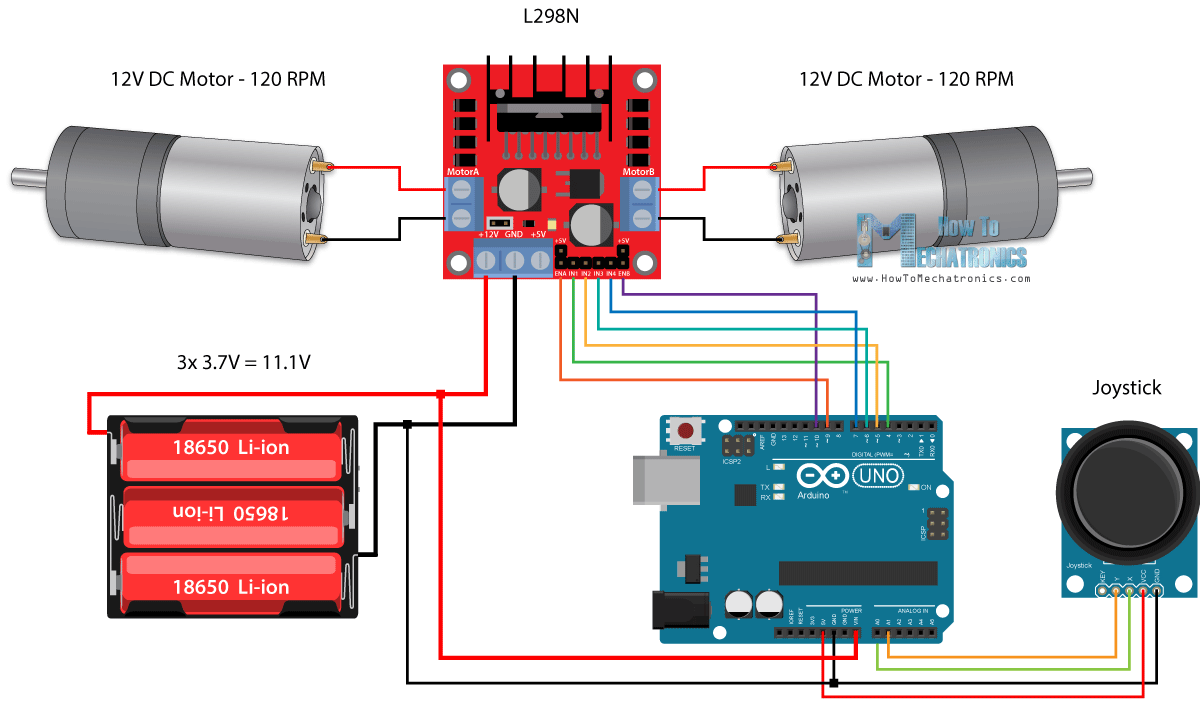
\includegraphics[width=0.5\textwidth]{./img/L298N.png}
\caption{馬達驅動器接線圖}
\label{fig:example}
\end{figure}
\begin{figure}
\centering
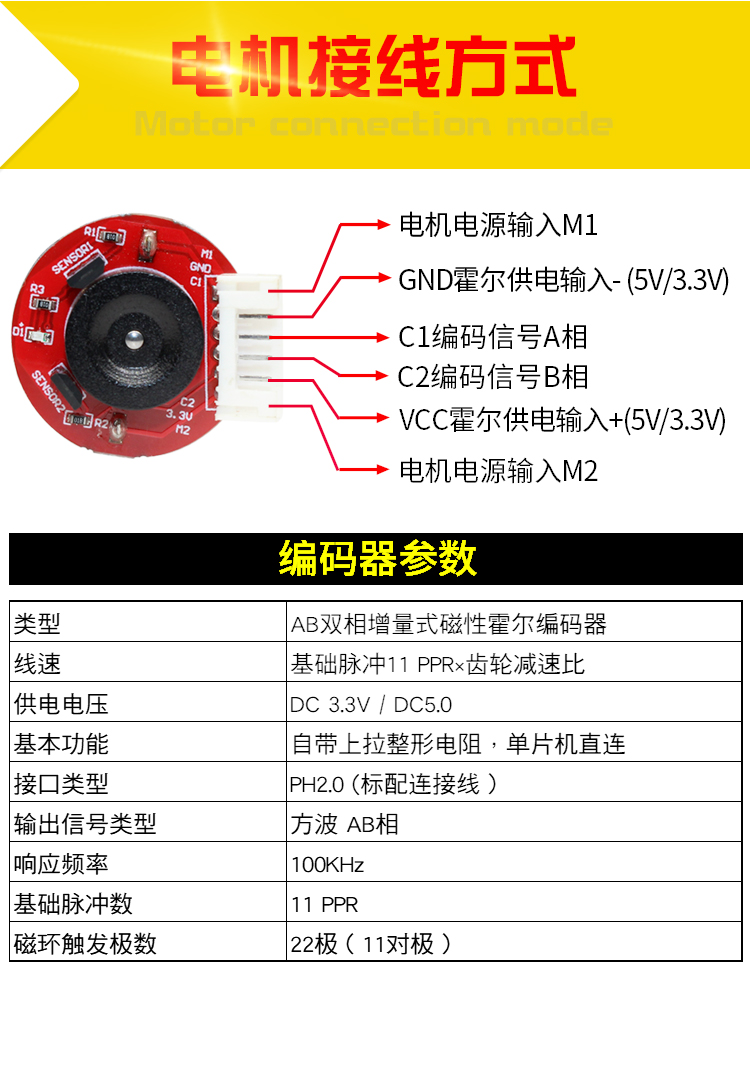
\includegraphics[width=0.5\textwidth]{./img/ZiWcCqr.png}
\caption{霍爾傳感器}
\label{fig:example1}
\end{figure}

\begin{figure}[htp]
\centering
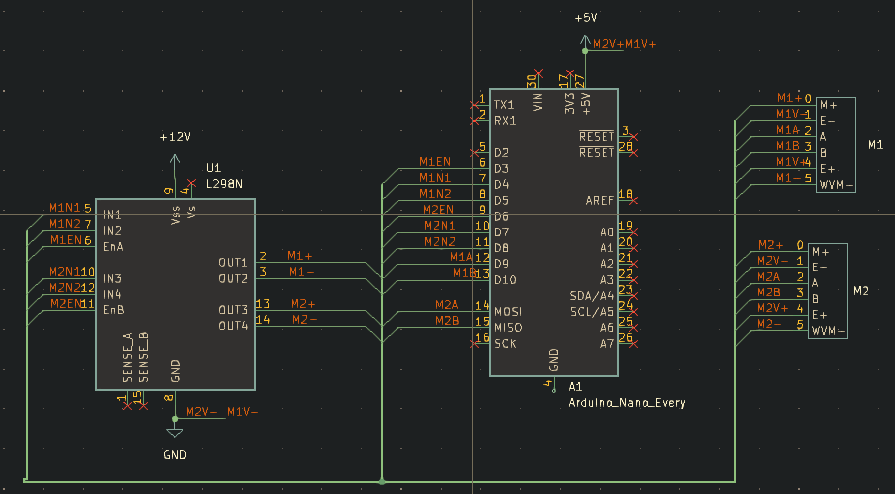
\includegraphics[width=1\textwidth]{./img/arduino.png}
\caption{電路接線圖}
\label{fig:example2}
\end{figure}


\subsection{電路接法}
如圖\ref{fig:example}是驅動器的接線方式,
如圖\ref{fig:example1}是霍爾編碼器的接腳,
圖\ref{fig:example2}是arduino與編碼器跟驅動器的接線圖。
gpio的接腳可以由程式定義,基本上根據定義來接線,IMU的接法如
表\ref{tab:connection}接法一樣之後在把CP2104接到數梅派的USB就
可以用UART通訊讀取資料。
